% !TeX encoding = UTF-8
% !TeX spellcheck = en_US

\newcommand{\doublequotes}[1]{``#1''}
\newcommand{\reference}[1]{\ref{#1} \nameref{#1} (page \pageref{#1})}
\newcommand{\introreference}[1]{Chapter \ref{#1}: \nameref{#1} (page \pageref{#1})}

\documentclass[a4paper,oneside]{report}

\pdfminorversion=7
\pdfcompresslevel=9
\pdfobjcompresslevel=2

\usepackage[hidelinks]{hyperref}
\usepackage[margin=60pt]{geometry}
\usepackage[T1]{fontenc}
\usepackage[utf8]{inputenc}
\usepackage[english]{babel}
\usepackage{array}
\usepackage{colortbl}
\usepackage{enumitem}
\usepackage{fancyhdr}
\usepackage{graphicx}
\usepackage{minted}
\usepackage{xcolor}

\usemintedstyle{staroffice}

\arrayrulecolor{lightgray}
\def\arraystretch{1.2}

\setlength{\parindent}{0pt}

\hypersetup{
    pdftitle={GPU101 - SYMGS},
    pdfauthor={Pierluigi Negro}
}

\newcommand\nbvspace[1][3]{\vspace*{\stretch{#1}}}

\raggedbottom

\renewcommand{\headrulewidth}{0pt}

\fancypagestyle{plain}{
    \fancyhead{}
    \fancyfoot{}
}

\pagestyle{fancy}

\fancyhead{}
\fancyfoot{}

\renewcommand{\chaptermark}[1]{\markboth{#1}{#1}}


\begin{document}

    \begin{titlepage}

        \begin{center}

            \nbvspace[1]

            
\includegraphics[width=0.3\columnwidth]{./images/polimi}

            \nbvspace[2]

            {\huge \textbf{\textsc{GPU101 - SYMGS}}} \\
            [1.5em]
            {\Large Report}

            \nbvspace[8]

            \Large \textbf{Pierluigi Negro}

            \nbvspace[2]

            \today \\ [0.5em]

            \nbvspace[1]


        \end{center}

    \end{titlepage}

    \pagebreak

    \chapter*{Introduction}
    
    \large 
    This project focuses on implementing in CUDA programming language a variant of the SYMGS algorithm, provided in its CPU implementation in the file \doublequotes{symgs-csr.c} contained in folder \doublequotes{symgs}, developed by professor Alberto Zeni. 
    
    The GPU implementation has to provide a time improvement over the CPU implementation. Time for the GPU implementation is calculated by registering the time before the first kernel call and after the last kernel call: large memcopies are excluded. Time for the CPU implementation is calculated by registering the time before and after the only function call. The correctness of the program is evaluated by comparing the elements of the result vector \verb|x|.

    All computations and times have been executed and taken on the architecture present on my computer. I have an \doublequotes{Intel Core i7 (7th generation)} CPU and an \doublequotes{NVIDIA 1050 GEFORCE GTX} GPU.

    The final file is the file \doublequotes{final.cu} contained in the main branch. Compile it using the command \verb|nvcc -o output final.cu -O3| from terminal. Run it by calling the output file and the path to the input matrix: \verb|./output /directory/kmer_V4a.mtx|.
        
    \begingroup
    \let\clearpage\relax
    \chapter*{Implementation}
    \endgroup

    \section*{Assumptions}

    In implementing the SYMGS algorithm I made a few assumptions regarding the dataset used, specifically: 
    \begin{itemize}
        \item All the input needed for the algorithm can reside inside the device's global memory
        \item All the input needed is correct
    \end{itemize}
    The first assumption proved to be true for my GPU architecture, while the second assumption was not. The array \verb|int col_ind[]|, which contains the indices of the non-zero values of the matrix, includes a -1 value. Using this value for indexing the \verb|x| vector could and did result in accessing memory outside the allocated space, making the algorithm not behave as intended. Luckily a simple check solved this issue. Another problem regarded the array \verb|float x[]|. Each element in the array is generated by the division of two random integers. The problem encountered revolved around the fact that the division of two integers yields an integer result, that cast to a float is represented as an integer with leading zeros. This messed with the arithmetic done inside the GPU, which treated these numbers as integers and was stuck with integer arithmetic: the output vectors remained integers. I fixed this problem directly in the creation of the vector, by casting the random integers to float and then dividing them, therefore yielding a float number. I took the liberty of doing this since it both solved my problem and looked like it was the intention of dividing two numbers in the first place. 
    
    \section*{Algorithm}

    The implementation allocates these arrays in the device's global memory:
    \begin{itemize}
        \item \verb|int* row_ptr|
        \item \verb|int* col_ind|
        \item \verb|float* values|
        \item \verb|float* x|
        \item \verb|float* matrixDiagonal|
        \item \verb|float* x2|
        \item \verb|char* locks|
        \item \verb|char* thread_done|
    \end{itemize}
    and a single \verb|char not_done|, used as a boolean value.

    After executing all the necessary mallocs and memory copying, the program divides into two sections that execute the forward and backward sweep of the algorithm. Both sections undergo the same steps but call the respective forward and backward kernel functions. The \doublequotes{sweep} is divided into \doublequotes{callsn} sections, which are approximately equal in length regarding the number of elements of x calculated. Each section is rerun until all values relative to that section are found.

    Having defined parameters at the start, each kernel thread has to solve for \verb|LINESPERTHREAD| number of lines (typically 8). Since the number of threads in a block is also fixed with \verb|THREADN|, the only way to cover all lines is to change the number of blocks needed. The last block likely has some threads that would try to access unallocated memory, since all lines might be already covered in other threads. Therefore, a check is done at the beginning of each kernel function to return right away in these cases. Following this check, the kernel checks if all values for that index have already been calculated using \verb|thread_done[]| from global memory, since the same values are to be calculated by the thread having the same index, and the index derives from the \verb|blockId| and the \verb|threadId|. If they have, the kernel returns right away. Then a loop is conducted over the number of lines to calculate. For each line it checks if the value has already been calculated, using \verb|locks[]| from global memory, skipping the line if it was. Then it starts doing multiplications using numbers contained in \verb|values[]| and in \verb|x| or in \verb|x2|, depending on if values were to be already calculated or not. Before grabbing elements from the array containing the new values, it checks if these values were already calculated using \verb|locks[]|. If they weren't, it skips the line and sets not done to 1. If all new values were already calculated, the resulting new value is inserted into the new value array and the corresponding lock is updated. If no line was skipped due to missing values, the corresponding \verb|thread_done| is set to 1 or 2 (forward or backward sweep), allowing the thread to exit right away in the next iteration. By resetting not done to 0 before every iteration of the same \doublequotes{chunk}, we can check after the kernel execution if all new values were calculated by evaluating not done: if it was set to 1 the program needs to iterate again, otherwise, the next chunk can be executed.

    At the end of the backward sweep, \verb|memcopy| is executed to copy the resulting vector into the host memory, in order to compare the results found by the GPU against the ones found by the CPU. Since these results varied ever so slightly, errors are defined both by arithmetical distance and by percentage, since there did not seem to be a way to have greater precision over them.
    
    


    \chapter*{Profiling}

    I checked the correctness and efficiency of my program by using tools such as \verb|cuda-memcheck| and \verb|nvvp|. The first tool is used when calling the executable from the command line and is useful to discover mistakes in memory access. In particular, if the executable was compiled with the \verb|-G| flag, it specifies the line of the mistake.

    The second tool, from which the two following figures are taken, was used to check for bottlenecks at execution time. In particular, the idea of dividing the two sweeps into chunks derived from seeing how much useless computation was spent on returning early after the initial bunk computation. In Figure 2 we can see that not a lot of time is spent on successive calls to the kernel function. Also, by using this tool I discovered that the matrix used as the dataset is lower triangular, making the use of chunks for the backward sweep useless but not tolling.

    \begin{figure}[h!]
        \centering
        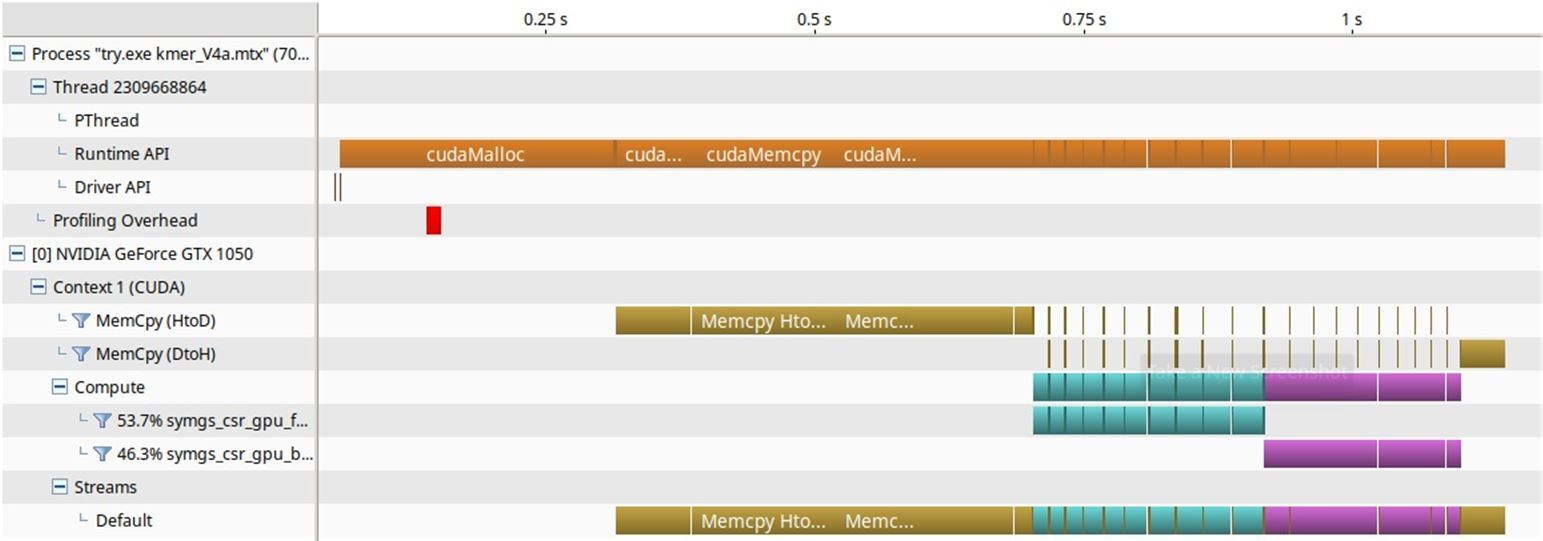
\includegraphics[width=1\columnwidth]{./images/whole-T}
        \caption{profiling of most of the program as seen from API calls. The colors, from top to bottom, represent API calls in orange, Memcopies in brown, kernel forward sweep in blue, kernel backward sweep in pink.}
    \end{figure}

    \begin{figure}[h!]
        \centering
        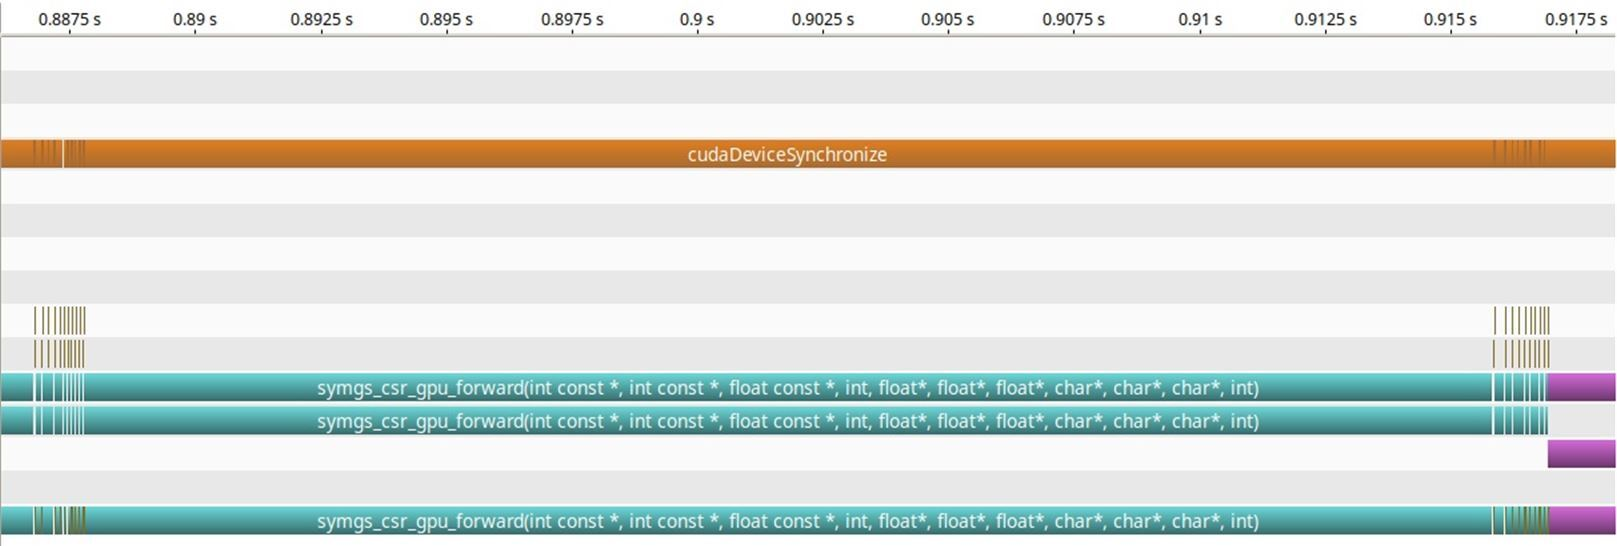
\includegraphics[width=1\columnwidth]{./images/forward-T}
        \caption{detail of Figure 1, last chunk of the forward sweep.}
    \end{figure}
    
    
    \begingroup
    \let\clearpage\relax
    \chapter*{Comments}
    \endgroup
    
    Using my GPU architecture, the GPU implementation seemed to improve the time taken by 30-50\%, ignoring the time taken by memory transfers to and from the device. Time could be further improved using a different GPU architecture as it strongly relies on how many blocks can be run simultaneously: given my architecture and the parameters present in the program, at most two blocks can run simultaneously.

    The program could be further improved by making use of shared memory or warp speed, but I did not manage to get significant results when trying to implement it using these techniques.

    The programs that lead up to the final results can be found in the repository by traversing the tree of commits, in the file \doublequotes{comparison.cu} in the folder \doublequotes{symgs}. This file can still be seen as a debug version of the final result.

    The idea to divide the sweeps into chunks and to execute those chunks until all values were found proved to be effective in reducing the time needed and overcoming the obstacle of dependencies between rows, but is not needed in the backward sweep since no dependencies are present. 

\end{document}